\chapter{Sicurezza dei sistemi e permessi}

\section{Introduzione}
La sicurezza nei sistemi differisce rispetto alla sicurezza delle reti, in quanto:
\begin{itemize}
    \item Possibilità di avere un ente certificato nel mezzo (Sistema operativo);
    \item I sistemi possono essere singolo o multi-utente;
    \item Possibilità di divisione dei privilegi.
\end{itemize}
È quella su cui agiscono Malware locali.

\subsection{Privilege Escalation}
Si definisce \textbf{Privilege Escalation} la possibilità di ottenere più privilegi sul sistema.
Ad esempio la possibilità di installare programmi, leggere informazioni private o
modificare configurazioni del sistema.

\section{Arbitrary Code Execution}
Il primo passo per eseguire un privilege escalation è l'esecuzione arbitraria di codice (e.g. per poter effettuare attacchi per ottenere privilegi più elevati).
Vi sono vari modi per perpetrare questa strada:
\begin{itemize}
    \item installando software;
    \item facendo girare software;
    \item sfruttando vulnerabilità in grado di dirottare il funzionamento dei programmi.
\end{itemize}

\section{Come funziona Unix}
In Unix la maggior parte delle risorse funziona come un file, questo significa che ottenendo l'accesso a un file potremo ottenere a sua volta l'accesso alla risorsa stessa, (e.g. /dev/snd/* per l’audio).

Il sistema mantiene le informazioni di accesso a un file tramite un meccanismo denominato \textbf{ACL (Access Control List)}. Queste vengono rappresentate come una tabella soggetto-oggetto, (e.g. Alice: read,write; Bob: read; Other: read). Normalmente Linux/Unix dichiara 3 oggetti:
\begin{itemize}
    \item il proprietario di un file;
    \item il gruppo proprietario di un file;
    \item tutti gli altri.
\end{itemize}
\clearpage
I soggetti sono identificati tramite un file (/etc/passwd) il quale contiene un'associazione nome utente: user id. Lo user id viene quindi salvato nel filesystem, associato ad ogni file.
\begin{figure}[h!]
    \centering
    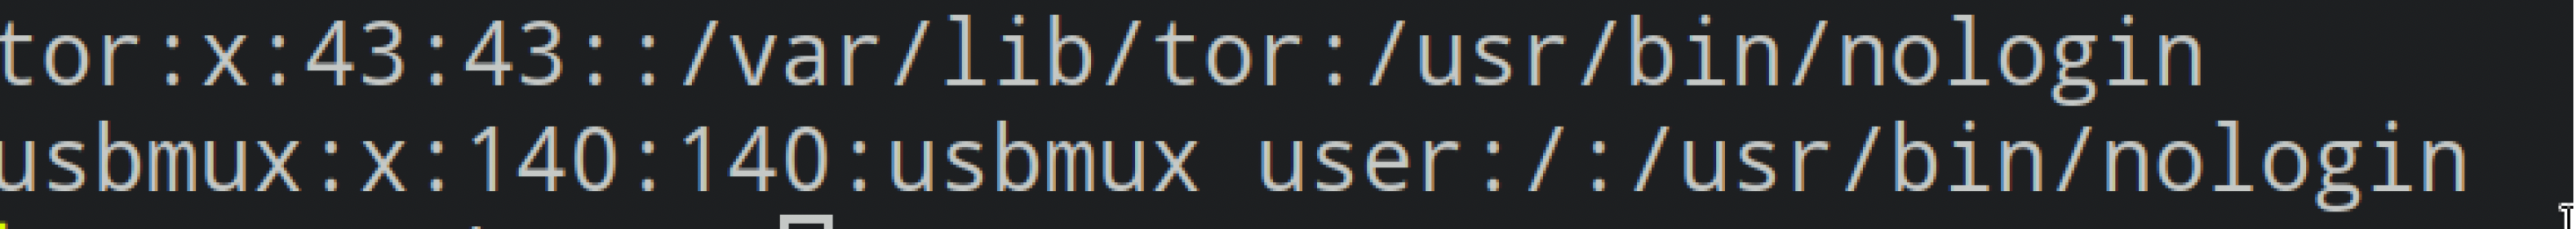
\includegraphics[width=.6\linewidth]{res/user_id.png}
    \caption{}
\end{figure}\\
Analogamente esiste un file anche per i gruppi (/etc/group) e un group id per gruppo.
\begin{figure}[h!]
    \centering
    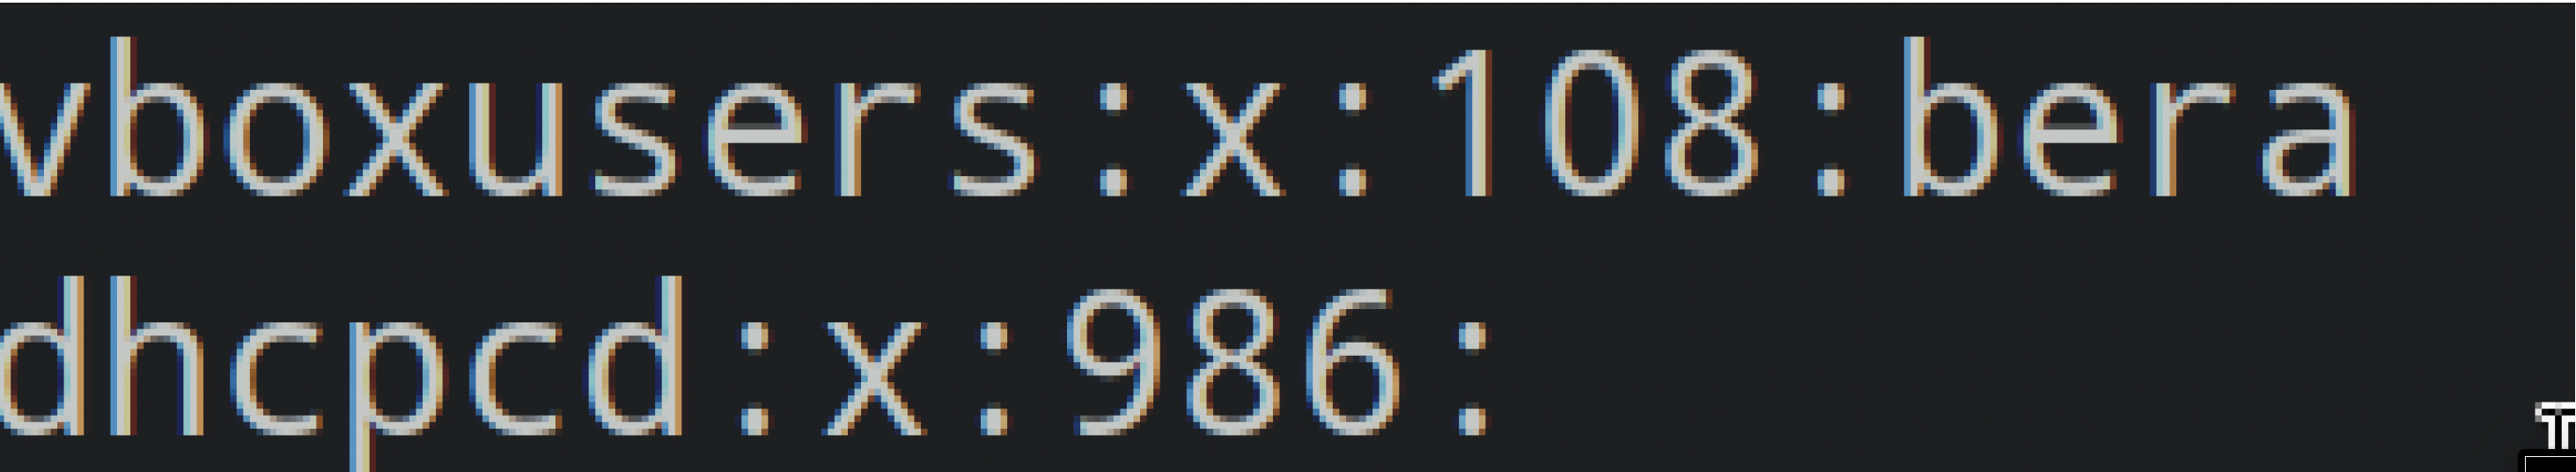
\includegraphics[width=.4\linewidth]{res/group_id.png}
    \caption{}
\end{figure}
Normalmente un Unix (sistemi multi-utente) è possibile "regalare" l'accesso a file ad altri utenti mediante in comando \textit{chmod} (che vedremo in seguito).

\section{Capabilities}
Una capability è un token in grado di rappresentare un determinato oggetto a cui si ha accesso. Alcuni esempi di capability sono: 
\begin{itemize}
    \item i cookie web, identificatori che indicano a quale sessione è associata una comunicazione;
    \item i file aperti.
\end{itemize}
A seguito di una system call di tipo open, viene ritornato un identificativo unico che verrà riconosciuto dal sistema operativo per indicare il file.
\begin{figure}[h!]
    \centering
    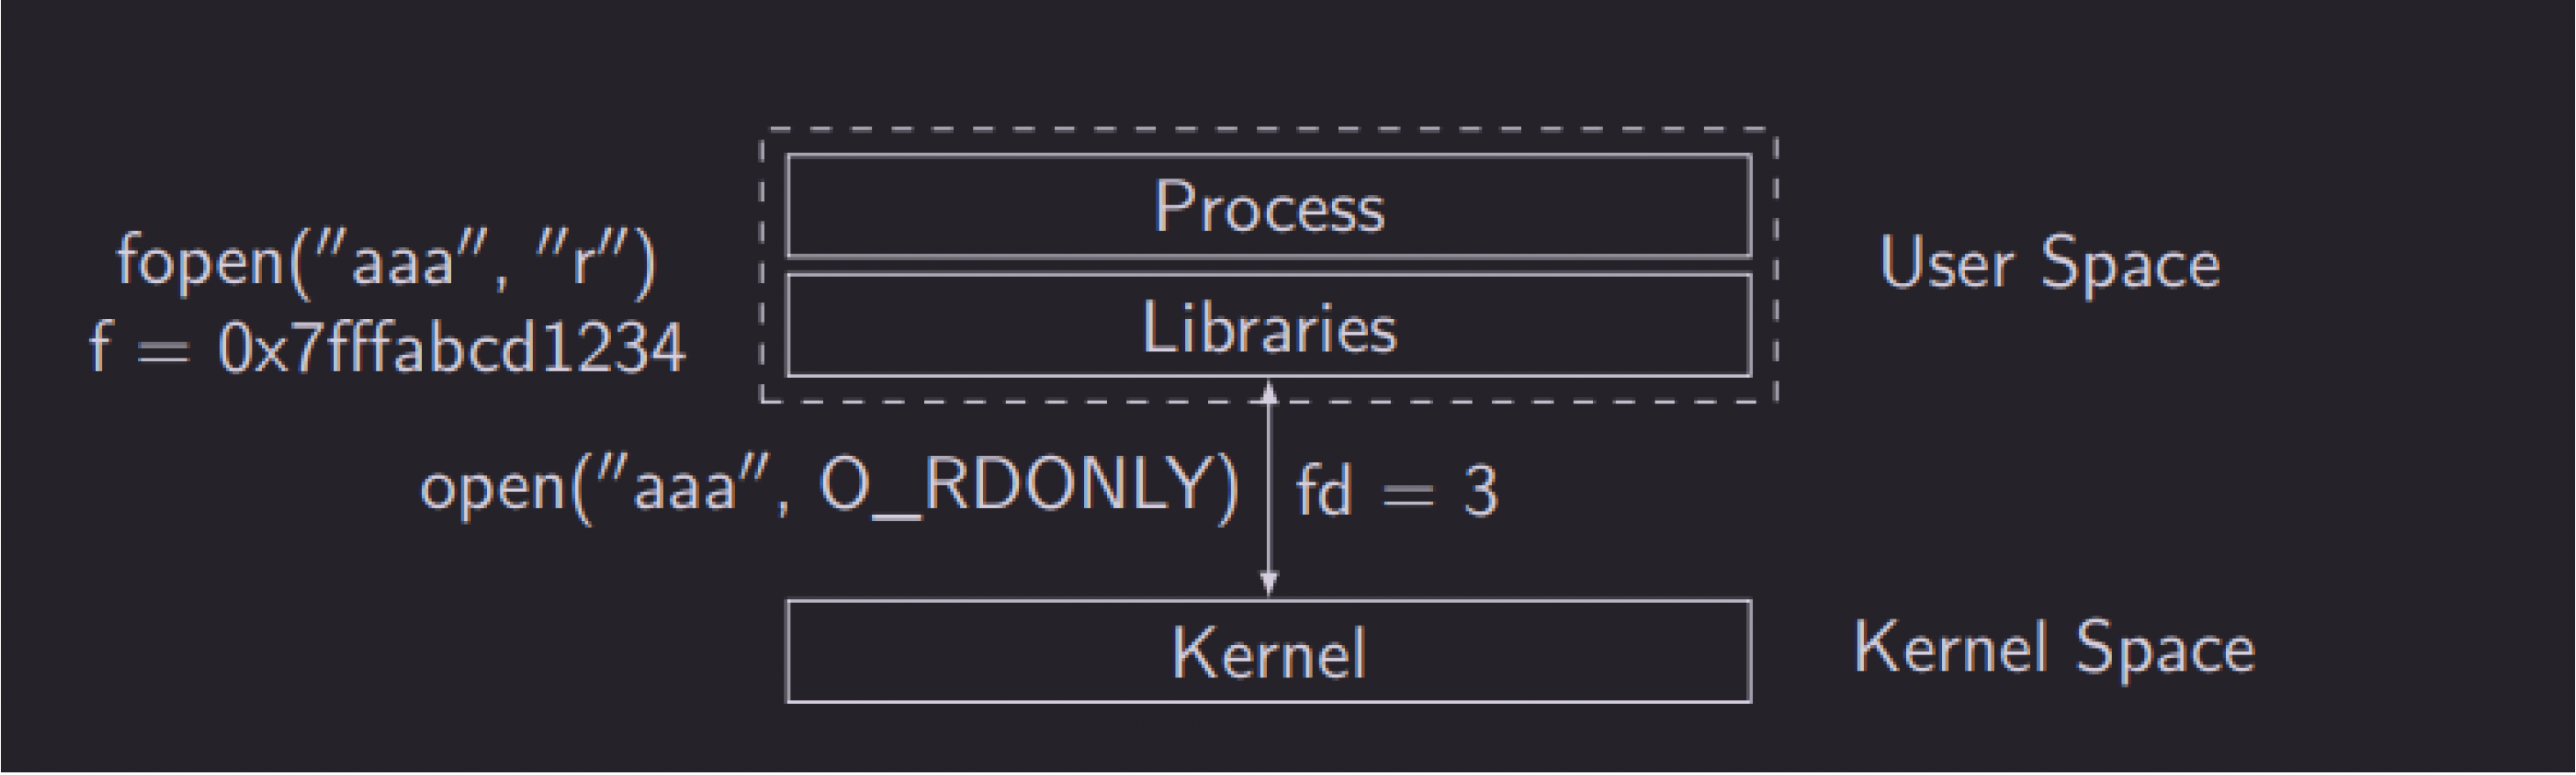
\includegraphics[width=.6\linewidth]{res/capabilities.png}
    \caption{}
\end{figure}
Le capability posso essere supportate da sistemi crittografici (e.g. cookie) oppure da segmentazione a livello di sistema operativo (e.g. file).
Unix in particolare utilizza una misto tra ACL (file non aperti) e capabilities (file aperti, socket, ecc.).

\section{Modelli di scambio delle informazioni}

\subsection{MAC}
Per evitare il "regalo" di accesso da parte dell'utente owner è possibile utilizzare un sistema di \textbf{MAC (Mandatory Access Controll} (in linux ne esistono diversi: SeLinux, Tomoyo, SMACK, ecc.), è facile pensare a questi sistemi come nel caso della segregazione delle applicazioni Adnroid (e.g. da telegram non posso accedere ai messaggi di whatsapp).

\subsection{Modello Bell-LaPadula}
Esistono diversi modelli di flusso per le informazioni. Supponiamo di avere diversi file a diversi livelli di segretezza. Il modello Bell-LaPadula mette in atto le seguenti regole:
\begin{itemize}
    \item ogni soggetto e ogni oggetto hanno un livello di segretezza;
    \item un soggetto può leggere oggetti a livello di sicurezza minori o uguali al suo;
    \item un soggetto può scrivere oggetti a livelli di sicurezza pari o maggiori del suo. 
\end{itemize}
Questo metodo viene classificato come WURD, Write Up Read Down.

Supponiamo di avere tre livelli di sicurezza: Top-Secret, Secret, Public.
Alice è un' operatrice di livello Secret. Alice quindi potrà:
\begin{itemize}
    \item leggere documenti di livello Secret e Public;
    \item scrivere documenti di livello Secret e Top-Secret.
\end{itemize}
Alice quindi non potrà né scrivere documenti di livello Public né leggere documenti di livello Top-Secret.

\subsection{Modello Biba}
Al contrario di Bell-LaPadula Biba è un modello duale a esso, mettendo in atto le seguenti regole:
\begin{itemize}
    \item ogni soggetto e ogni oggetto hanno un livello di segretezza;
    \item un soggetto può scrivere oggetti a livelli di sicurezza pari o minori al suo;
    \item un soggetto può leggere oggetti a livelli di sicurezza pari o maggiori al suo.
\end{itemize}
Questo metodo viene classificato come WDRU, Write Down Read Up, metodo particolarmente utilizzato per l'integrità delle informazioni. Nel mondo Windows questo metodo prende il nome di Integrity Level (IL).

Supponiamo di avere tre livelli di sicurezza: Capitano, Tenente, Carabiniere Scelto.
Alice è un'operatrice a livello Tenente. Alice quindi potrà:
\begin{itemize}
    \item leggere documenti rilasciati da Tenenti e Capitani;
    \item scrivere documenti per Tenenti e Carabinieri Scelti
\end{itemize}
In questo modo si garantisce l'integrità delle informazioni non dando la possibilità di dare ordini a un suo superiore.
\section{Filesystem}
Nei sistemi operativi il sistema per lo scambio dei dati locali è il filesystem.
\clearpage
\begin{center}
    \begin{table}[]
        \centering
        \begin{tabular}{|c|c|}
            / & The root filesystem \\
            /proc & (pseudo) The process virtual infrastructure (e.g. /proc/1/cmdline) \\
            /sys & (pseudo) The system virtual infrastructure (e.g. /sys/class/leds) \\
            /dev & (pseudo) Device drivers file interface (e.g. /dev/sda) \\
            /run &  (pseudo) Contains run-time information \\
            /etc & Configuration directory \\
            /tmp & Temporary directory, volatile, usually mount on RAM \\
            /root & Root's home \\
            /bin & Binaries \\
            /lib & Libraries \\
            /sbin & System binaries \\
            /usr & User binaries \\
            /var & Log, cache and structured personal files (e.g. mailbox) \\
            /home & User's directory \\
            /mnt & External mountpoint \\
            /opt & Optionals softwares \\
        \end{tabular}
        \caption{Esempio filesystem Linux}
    \end{table}
\end{center}
Come dichiarato precedentemente il sistema in modalità DAC analizza in questo ordine i vari permessi, seguendo il seguente ordine:
\begin{enumerate}
    \item UID processo e proprietario del file;
    \item GID e gruppo del file;
    \item UID e Other.
\end{enumerate}
Questa modalità di analisi può generare complicanze contro-intuitive (esempio se l’utente appartiene a un gruppo che può leggere il file ma è il suo proprietario e il proprietario non può leggere il file).
Il super utente privilegiato del sistema (superuser) è l'unico che può svolgere ogni operazione a partire dalla radice (root, in ambienti Linux/Unix) del filesystem.
\'E possibile assegnare un file anche a una persona diversa, soltanto l'utente root di norma potrà "regalare" i file a chiunque.
All'occorrenza è possibile anche cambiare i permessi associati a un file, mediante il comando \textit{chown}. Questo comando prevede un interfaccia a linea di comando in grado di interpretare numeri in base 8 (ottali) o attraverso un sistema di configurazione più "intuitivo" basato su un linguaggio specifico:
\begin{itemize}
    \item bit 0: execute, possibilità di eseguire il file;
    \item bit 1: write, possibilità di scrivere il file;
    \item bit 2: read, possibilità di leggere il file.
\end{itemize}
Come possiamo intuire, impostando come permessi la terzina, 777, ci troveremo a "regalare" l'accesso al file a chiunque creando problemi di sicurezza (other: read, write, execute).

Sulle cartelle i permessi differiscono dai permessi sui file:
\begin{itemize}
    \item bit 0: execute, possibilità di entrare in una cartella;
    \item bit 1: write, possibilità di eliminare i file contenuti in una cartella (anche quelli creati da un altro utente);
    \item bit 2: read, possibilità di leggere il contenuto di una cartella.
\end{itemize}
Anche in questo caso si potrebbe generare una security by obscurity in quanto se a una cartella assegniamo con il comando \textit{chmod} i permessi, 711, otterremo che il proprietariò potrà effettuare tutte le operazioni sulla cartella, mentre gli altri potranno accedere lo stesso alla cartella ma non loro caso non vedranno nessun file all'interno (security by oscurity).

Per com'è pensato il sistema un utente può appartenere a più gruppi, questa possibilità si usa principalmente gli accessi ai file per i device driver.

\begin{lstlisting}[language=bash]
    command:
    ls -la /dev/tty0

    output: 
    crw--w---- 1 root tty 4, 0 Mar 23 16:25 /dev/tty0
\end{lstlisting}

Esistono anche i permessi speciali su Linux salvati nei bit più significativi dei metadati del file (se usati male, molto pericolosi): 
\begin{itemize}
    \item setuid: se il file ha il flag impostato, il kernel avvia il processo relativo con i privilegi dell’utente proprietario del file piuttosto che con quelli dell’utente che lo ha lanciato in esecuzione, questo bit non ha effetto sulle cartelle;
    \item setgid, se una directory ha il flag impostato questa assegnerà ai file creati al suo interno il gruppo d’appartenenza della cartella, utile per mantenere all’interno di una cartella il gruppo corretto per tutti i file, un file eseguito con questo bit eseguirà con il gruppo di appartenenza;
    \item sticky: se impostato il flag essa permetterà l’eliminazione dei file al suo interno solo al suo owner (anche se la cartella ha permesso di scrittura per tutti, e.g. /tmp/), su un file lo sticky bit è ignorato e deprecato.
\end{itemize}
Ciò rende l'utilizzo di questi bit \textbf{estremamente pericoloso}.

\begin{ex}
    Cosa succede, ad esempio se usiamo il seguente codice C?
    
    \begin{lstlisting}[language=C]
        ...
        system("whoami");
        ...
    \end{lstlisting}
    
    Otterremo l'esecuzione del comando \textit{whoiam} con i privilegi dell'utente indicato, essendo un comando shell, questo potrà essere dirottato per eseguire del codice malevolo.

    \begin{lstlisting}[language=bash]
        PATH=. ./vulnprogram
    \end{lstlisting}
\end{ex}
Proprio sfruttando questa escalation di privilegi il comando \textit{sudo} pone il suo funzionamento, ponendosi con privilegi elevati e controllando la password dell'utente.
Essendo \textit{setuid} un chiaro problema di sicurezza, in quanto per ottenere i privilegi di root e.g. per cambiare un file otterremo l'intero insieme di privilegi (e.g. la possibilità di cambiare indirizzo IP della macchina), per questo motivo si è pensato bene di spezzettare i vari privilegi in modo tale da assegnare solo quelli che servono per la corrente esecuzione, (e.g. CAP\_NET\_ADMIN, CAP\_DAC\_OVERRIDE, per altri basta consultare il manuale delle capabilities).
